
\documentclass[12pt]{article}
\usepackage[spanish]{babel}
\usepackage{booktabs}
\usepackage{longtable}
\usepackage{latexsym}
\usepackage{lipsum}
\usepackage{graphicx}
\usepackage{xcolor}
\usepackage{setspace}

\textwidth     =  6.5in
\textheight    =  9.0in
\oddsidemargin =  0.2in
\topmargin     = -0.6in
\usepackage{amsmath, amssymb, latexsym}


%%%%%%%%%%%%%%%%%%%%%%%%%%%%%%%%%%%%%%%%%%%%%%%%%%%%%%%%%%%%%%%%%%%%%%%%
\newcommand{\be}{\begin{equation}}
\newcommand{\ee}{\end{equation}}
\newcommand{\bes}{\begin{equation*}}
\newcommand{\ees}{\end{equation*}}

\newcommand{\bea}{\begin{eqnarray}}
\newcommand{\eea}{\end{eqnarray}}

\newcommand{\beas}{\begin{eqnarray*}}
\newcommand{\eeas}{\end{eqnarray*}}

\newcommand{\bet}{\begin{tabular}}
\newcommand{\ent}{\end{tabular}}
\newcommand{\mul}{\multicolumn}
\newcommand{\bec}{\begin{center}}
\newcommand{\enc}{\end{center}}
\newcommand{\bei}{\begin{itemize}}
\newcommand{\eni}{\end{itemize}}
\newcommand{\bee}{\begin{enumerate}}
\newcommand{\ene}{\end{enumerate}}
\newcommand{\noi}{\noindent}
\newcommand{\unl}{\underline}
\newcommand{\ul}{\underline}
\newcommand{\real}{\mathbb{R}}
\newcommand{\feal}{\mathbb{F}}
\newcommand{\natu}{\mathbb{N}}
\newcommand{\fact}{\mathbb{X}}

\begin{document}

\title{Optimizaci\'on num\'erica}
\author{Proyecto final 2. MPI}
\date{ Santiago Novoa P\'erez. 8 de diciembre del 2015.}
\maketitle


\subsubsection*{Introducci\'on}
\noi Los m\'etodos de puntos interiores (MPI) representan una alternativa a los m\'etodos de conjunto para resolver problemas de optimizaci\'on no lineal con restricciones de desigualdad. Mientras que la dificultad de los m\'etodos como PCS est\'a en encontrar el conjunto de restricciones de desigualdad que son activas en la soluci\'on (que alcanzan la igualdad), los m\'etodos de puntos interiores abandonan tal b\'usqueda manteni\'endose siempre dentro de las regiones de desigualdad en lugar de avanzar por su frontera; esto se logra con diversas penalizaciones o barreras que se le agregan a la funci\'on a minimizar (por esto es que los m\'etodos de puntos interiores tambi\'en se conocen como m\'etodos de barrera). \\
 
  Los m\'etodos MPI tambi\'en resuelven una secuencia de subproblemas de optimizaci\'on (parecido a PCS en ese aspecto), sin embargo, lo \'unico que cambia entre subproblema y subproblema es el par\'ametro de penalizaci\'on (o el peso que se le da a la barrera sobre la funci\'on $\mu$), es decir, qu\'e tanto deja el m\'etodo a los valores reales acercarse a la frontera de las restricciones de desigualdad. Para alcanzar la soluci\'on al problema original se intenta avanzar tanto hacia la frontera como sea necesario (el parametro de penalizaci\'on $\mu$ deber\'ia tender a cero para que el m\'etodo se aproxime a la soluci\'on).\\
  
   MPI es apropiado para problemas grandes y peque\~nos con funciones no lineales; en estos casos la soluci\'on se alcanza en un n\'umero de iteraciones sustancialmente menor que $n$.\\
   
  Nuestro enfoque para el m\'etodo (aunque no es el \'unico) ser\'a resolver el sistema de KKT de cada subproblema transformando al sistema de tal manera que tengamos las condiciones necesarias (simetr\'ia y curvatura positiva) para usar el algoritmo ldl (el cual nos deja usar la estructura de la matriz en la resoluci\'on de cada subproblema sin necesidad de calcular bases de espacios nulos ni matrices inversas paso a paso).\\
   
   Una vez resuelto el sistema para una $\mu$ se actualizar\'a el par\'ametro (reduci\'endolo en .1) y se volver\'a a calcular el sistema de KKT correspondiente. Es importante que al actualizar el par\'ametro (ciclo externo) se elija comenzar el m\'etodo (resolver el sistema de KKT resulta en un m\'etodo iterativo que ser\'a nuestro ciclo interno) con ${x_0}^{k+1}$ , la aproximaci\'on inicial, siendo el valor de la soluci\'on del subproblema anterior (${x_*}^{k}$). Al hacer \'esto nuestro m\'etodo empezar\'a a converger de manera mucho m\'as r\'apida cada que actualicemos el par\'ametro de barrera $\mu$.\\
  
\subsubsection*{Historia}

Los m\'etodos de barrera para optimizaci\'on se desarrollaron en los a\~nos sesenta, pero su popularidad cay\'o en las siguientes dos d\'ecadas. El \'exito que tuvieron los m\'etodos de puntos interiores para programaci\'on lineal en los a\~nos noventa renov\'o el inter\'es en estos m\'etodos para el caso no lineal. Para finales de 1990, hab\'ia surgido una nueva generaci\'on de m\'etodos y software para programaci\'on no lineal. Los m\'etodos de puntos interiores a menudo son m\'as r\'apidos que  los m\'etodos de programaci\'on cuadr\'atica sucesiva en grandes problemas, sobre todo cuando el n\'umero de variables libres es grande. \footnote{Nocedal, Jorge, and Stephen Wright. Numerical optimization. Springer Science \& Business Media, 2006.}

  
    \subsubsection*{Construcci\'on del m\'etodo}
    \noi.\\
  El problema que buscamos resolver es:
  \beas
  {\text {minimizar}}\ &\ f(x)\\
  {\text {s.a.}}\ \ &\  h(x) = 0 \\
  &\  g(x)\leq 0  \\ \\
  f: \real^n &\longrightarrow \real \\
  h: \real^n &\longrightarrow \real^{m_{h}} \ \ \ \\
  g: \real^n &\longrightarrow \real^{m_{g}}\ \ \  \\
  \eeas
\ \ \ \ \ \ \ \ \ \ \ \ \ \ \ \ \ \hfill{\small{* f, h, g dos veces continuamente diferenciables }}\\ \\
 
 \noi Transformamos el problema para evitar adivinar las restricciones activas:
 \beas
  {\text {minimizar}}\ &\ \psi(x)= f(x)-\mu*\sum\ln(s_i)\\
  {\text {s.a.}} &h(x) = 0 \\
  &\ \ \ \ \ \ \ \ \ \   g(x)+s =0;  \ \ \ \ \ \ \ s\geq 0\\
  \eeas

La barrera de este problema (barrera logar\'itmica) evita que los valores de $s$ sean cero ya que penaliza demasiado a la funci\'on $\psi(x)$ para cualquier $s_i = 0$. De esta manera podemos resolver el sistema de KKT sin tener que preocuparnos por si estamos llegando a la frontera de las desigualdades. 		\\
  
  El siguiente paso a seguir ser\'ia encontrar los valores de (x,s) factibles que minimizan al problema. Como criterio se utilizan las condiciones de KKT.\\ \\
  \bei
\item{\it{C.N.P.O.}}
 \eni
 \noi Se buscan multiplicadores tales que en el minimizador local el gradiente de la funci\'on objetivo (en este caso la funci\'on de barrera $\psi(x)$) sea combinaci\'on lineal (con los multiplicadores $\lambda$ como coeficientes) de los gradientes de las restricciones y se mantenga factibilidad. Para esto primero definiremos la funci\'on $Lagrangiana$ del problema y cambiaremos ciertas variables para facilitar su uso:
 
  \begin{eqnarray} 
\qquad && \mathcal{L}(z,\lambda;\mu) = \phi_{\mu}(x) + \lambda_{h}^{T}h(x) +\lambda_{g}^{T}(g(x)+s)
\label{eq1:problema}
\end{eqnarray}

Donde $s > 0$ es un vector de variables de holgura, $z = (x, s)^t$ y $\mu > 0$ es el par\'ametro de barrera.\\
  
  A partir de esta funci\'on se pueden obtener las condiciones necesarias de primer orden (con las cu\'ales construiremos nuestro sistema de KKT):
  
  \beas
  \frac{\partial\mathcal{L}}{\partial x}  =& \nabla f(x) + A_h(x)^t*\lambda_h + A_g(x)^t*\lambda_g\\
  (donde\ A_h,\ A_g\ son&\ las\ Jacobianas\ de\ las\ restricciones\ h(x),\ g(x)) \\ \\
  \frac{\partial\mathcal{L}}{\partial s}  =& -\mu*S^{-1}e + \Lambda_ge\\
   \frac{\partial\mathcal{L}}{\partial \lambda_h} =& h(x)\\
    \frac{\partial\mathcal{L}}{\partial \lambda_g}  =& g(x)+s;
  \eeas

\noi Las C.N.P.O. nos indican que necesitar�amos igualar las cuatro derivadas de arriba a cero, sin embargo, vamos a resolver el sistema de KKT con iteraciones del m\'etodo de Newton por lo que para encontrar esa soluci\'on todav�a se necesitan las segundas derivadas de cada una de las ecuaciones anteriores con respecto a x, s, $\lambda_h$ y $\lambda_g$.\\ \\
\pagebreak
\bei
\item{\it{C.N.S.O.}}
\eni

\begin{equation}
\begin{bmatrix}
\nabla_{xx}^2 \mathcal{L}(z,\lambda;\mu) & 0 & A_h^T(x) & A_g^T(x)\\ 
0 & -\mu S^{-2}e & 0 & \mathbb{I} \\
A_h(x) & 0 & 0 & 0 \\
A_g(x) & \mathbb{I} & 0 & 0
\end{bmatrix} 
\begin{bmatrix}
d_x \\
d_s \\
d_{\lambda_{h}} \\
d_{\lambda_{g}}
\end{bmatrix}
= -
\begin{bmatrix}
\nabla f(x) + A_h(x)^t\lambda_h + A_g(x)^t\lambda_g \\ 
 -\mu S^{-1}e +\Lambda_ge\\
  h(x) \\
  g(x) + s \\
 \end{bmatrix}  
\end{equation} \\
$\lambda = \left[\lambda_h,\lambda_g\right]^t$
$$\iff$$\\
\begin{equation*}
\begin{bmatrix}
\nabla_{xx}^2 \mathcal{L}(z,\lambda;\mu) +A_h^t(x)(\lambda_h^{+}-\lambda_h) + A_g^t(x)(\lambda_g^{+}-\lambda_g)\\ 
 -\mu S^{-2}d_s + (\lambda_g^{+}-\lambda_g)\\
A_h(x)d_x \\
A_g(x)d_x +d_s
\end{bmatrix} 
= -
\begin{bmatrix}
\nabla f(x) + A_h(x)^t\lambda_h + A_g(x)^t\lambda_g \\ 
 -\mu S^{-1}e +\lambda_g\\
  h(x) \\
  g(x) + s \\
 \end{bmatrix}  
\end{equation*} \\
$$\iff$$\\
\begin{equation*}
\begin{bmatrix}
\nabla_{xx}^2 \mathcal{L}(z,\lambda;\mu) +A_h^t(x)(\lambda_h^{+}) + A_g^t(x)(\lambda_g^{+})\\ 
 S*(-\mu S^{-2}d_s + (\lambda_g^{+}))\\
A_h(x)d_x \\
A_g(x)d_x +d_s
\end{bmatrix} 
= -
\begin{bmatrix}
\nabla f(x) \\ 
 S*(-\mu S^{-1}e)\\
  h(x) \\
  g(x) + s \\
 \end{bmatrix}  
\end{equation*} \\
\beas
sust.\ {\hat{d_s}}=&S*d_s\\
\mu S^{-1}=&\Lambda_g\\
&\implies
\eeas

\begin{equation}
\begin{bmatrix}
\nabla_{xx}^2 \mathcal{L}(z,\lambda;\mu) & 0 & A_h^T(x) & A_g^T(x)\\ 
0 & S\Lambda_g & 0 & S \\
A_h(x) & 0 & 0 & 0 \\
A_g(x) & S & 0 & 0
\end{bmatrix} 
\begin{bmatrix}
d_x \\
\hat{d_s} \\
\lambda_{h}^{+} \\
\lambda_{g}^{+}
\end{bmatrix}
= -
\begin{bmatrix}
- \nabla f(x) \\ 
 \mu e \\
 - h(x) \\
 - g(x) - s \\
 \end{bmatrix}  
\label{eq:sistemaKKT}
\end{equation} \\
\noi Finalmente llegamos al sistema que se va a resolver paso a paso (ciclo interno) actualizando $(z,$$\lambda$$)$.
 $$z^{+} = z + \alpha_{z}d_s, \ \ \ \ \ \lambda^{+} = \lambda  + \alpha_\lambda d_\lambda$$\\
 
 Para la actualizaci\'on se cuida que ni $\lambda_g^{+}\leq0$ ni $s_{k+1}\leq0$ . A esto se le llama protecci\'on del m\'etodo de Newton.
\\
\pagebreak

Para el ciclo externo s\'olo es necesario, una vez llegado al punto m\'inimo, actualizar $\mu_{k+1} = \frac{\mu_k}{10}$ y repetir el procedimiento con $x_0^{k+1}=x_*^{k}$ y calculando la $\lambda$ por m\'inimos cuadrados:
$$A^t\lambda=-\nabla f(x)$$
$$\iff$$
$$\lambda =- (AA^t)^{-1}A\nabla f(x)$$

\subsubsection*{Pseudo-c\'odigo}
$$$$

{\setstretch{0.8}\color{gray}
I. Fase inicial \\

\hspace{2.5cm}Dar aproximaciones iniciales $x_0$, $s_0$; $\mu_0 = 1$\\

\hspace{2.5cm}Generar $\lambda_0$ por m\'inimos cuadrados.\\

\hspace{2.5cm} $k_{int} = 0$ y $k_{ext} = 0; fact = 0.1 $\\

II. Cuerpo \\

\hspace{2.5cm} While not(convergencia) \& $k_{ext} \le 10 $ \\

\hspace{5.5 cm} While not(convergencia BL) \& $k_{int} \le 100 $ \\

\hspace{7 cm} Construir la matriz de coeficientes K \\

\hspace{7 cm} if inercia\_correcta \\

\hspace{9 cm} Obtener $d_x, d_s, d_{\lambda_h}, d_{\lambda_g}$ \\

\hspace{9 cm} Obtener $\alpha_z, \alpha_\lambda$ y cortar pasos\\

\hspace{9 cm} Obtener $z^{+}$ y $\lambda^{+}$ \\

\hspace{9 cm} $k_ {int} = k_{int} + 1$; \\

\hspace{7 cm} else \\

\hspace{9 cm} print (inercia incorrecta) \\

\hspace{9 cm} end \\

\hspace{5.5cm} $k_ {ext} = k_{ext} + 1$; \\

\hspace{5.5cm} $\mu_ {k_{ext}} = {fact}*\mu_{k_{ext-1}}$; \\

\hspace{5.5cm} $x_0^{k_{ext}} = x_*^{k_{ext}-1}$; \\

\hspace{2.5cm} end 
}
\pagebreak
\subsubsection*{Ejemplos de funciones}
\begin{center}
\begin{figure}[h]
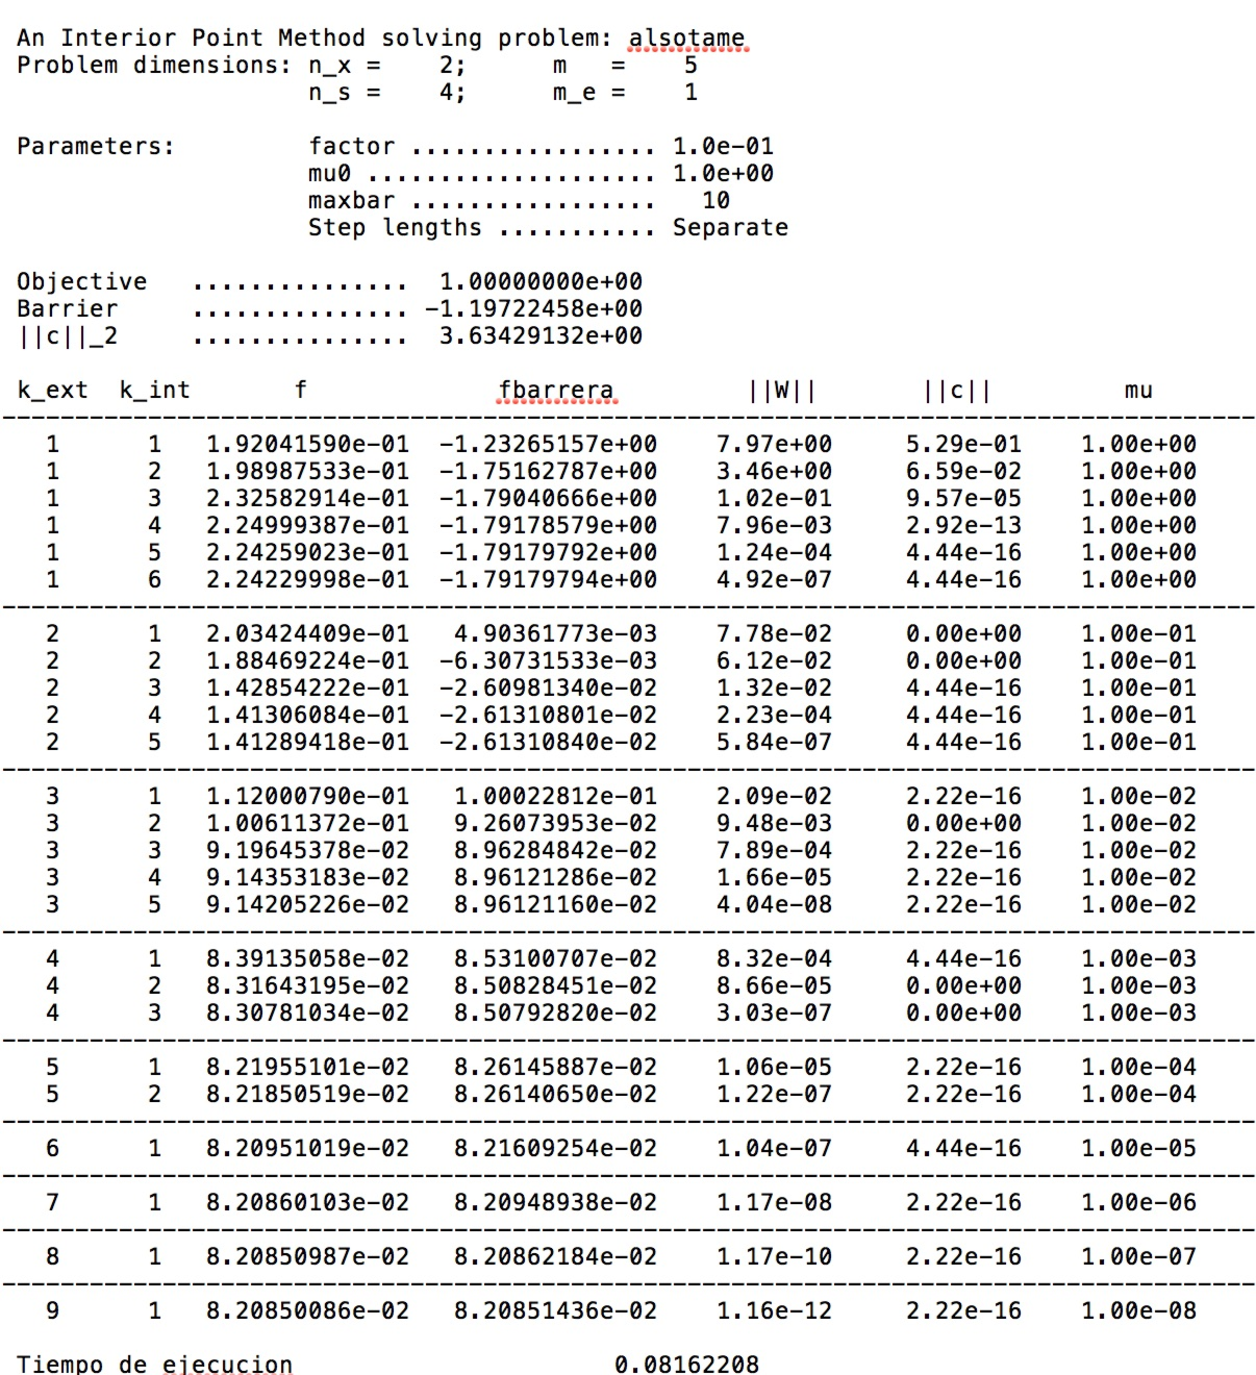
\includegraphics[trim=0 0 0 0,scale = 0.65]{alsotame}
\end{figure}
\end{center}
\bei
\item Podemos ver que conforme va avanzando el m\'etodo el n\'umero de iteraciones dentro de cada ciclo interno va disminuyendo de manera muy importante.
\eni
\pagebreak
\begin{center}
\begin{figure}[h]
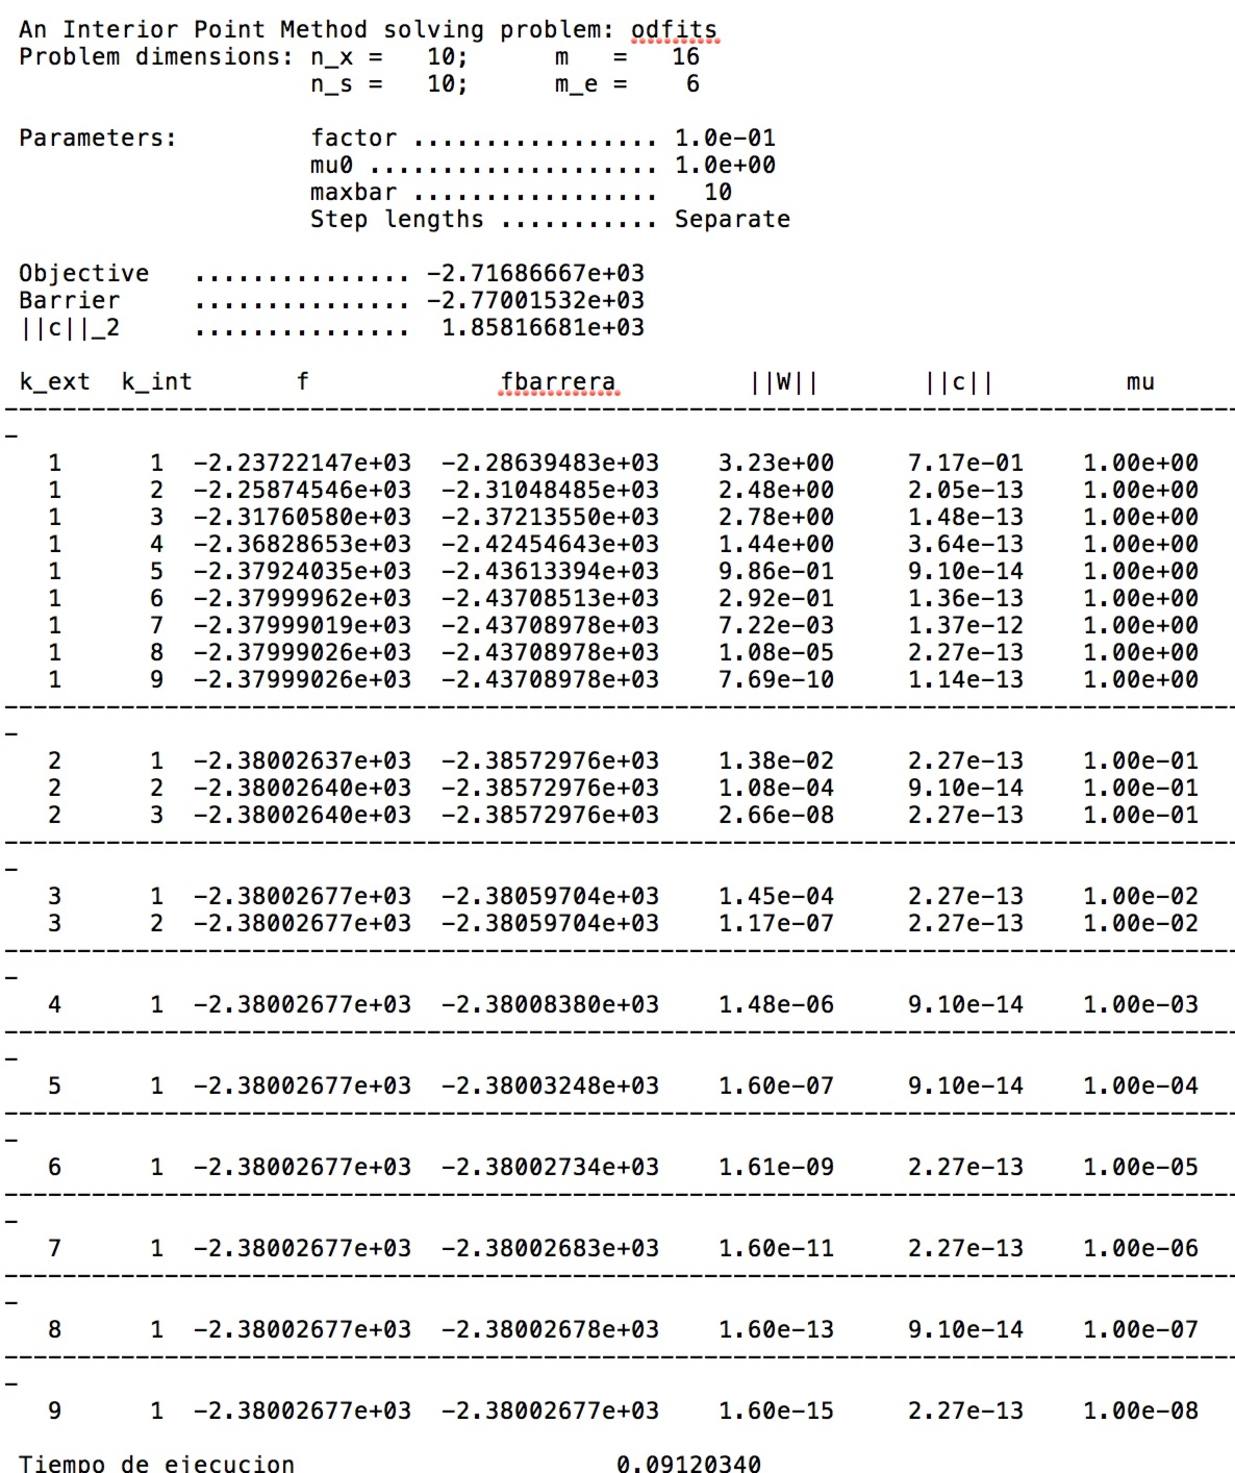
\includegraphics[trim=0 0 0 0,scale = 0.65]{odfits}
\end{figure}
\end{center}
\bei
\item Adem\'as, el intercambio entre $\|W\|$ y $\|c\|$ es mucho menor en las primeras iteraciones que en las finales, esto tambi\'en se debe al tipo de convergencia que hay al principio del algoritmo y c\'omo \'este se acelera conforme va acerc\'andose a la vecindad del m\'inimo (conforme se va acercando a la frontera).
\eni
\pagebreak
\begin{center}
\begin{figure}[h]
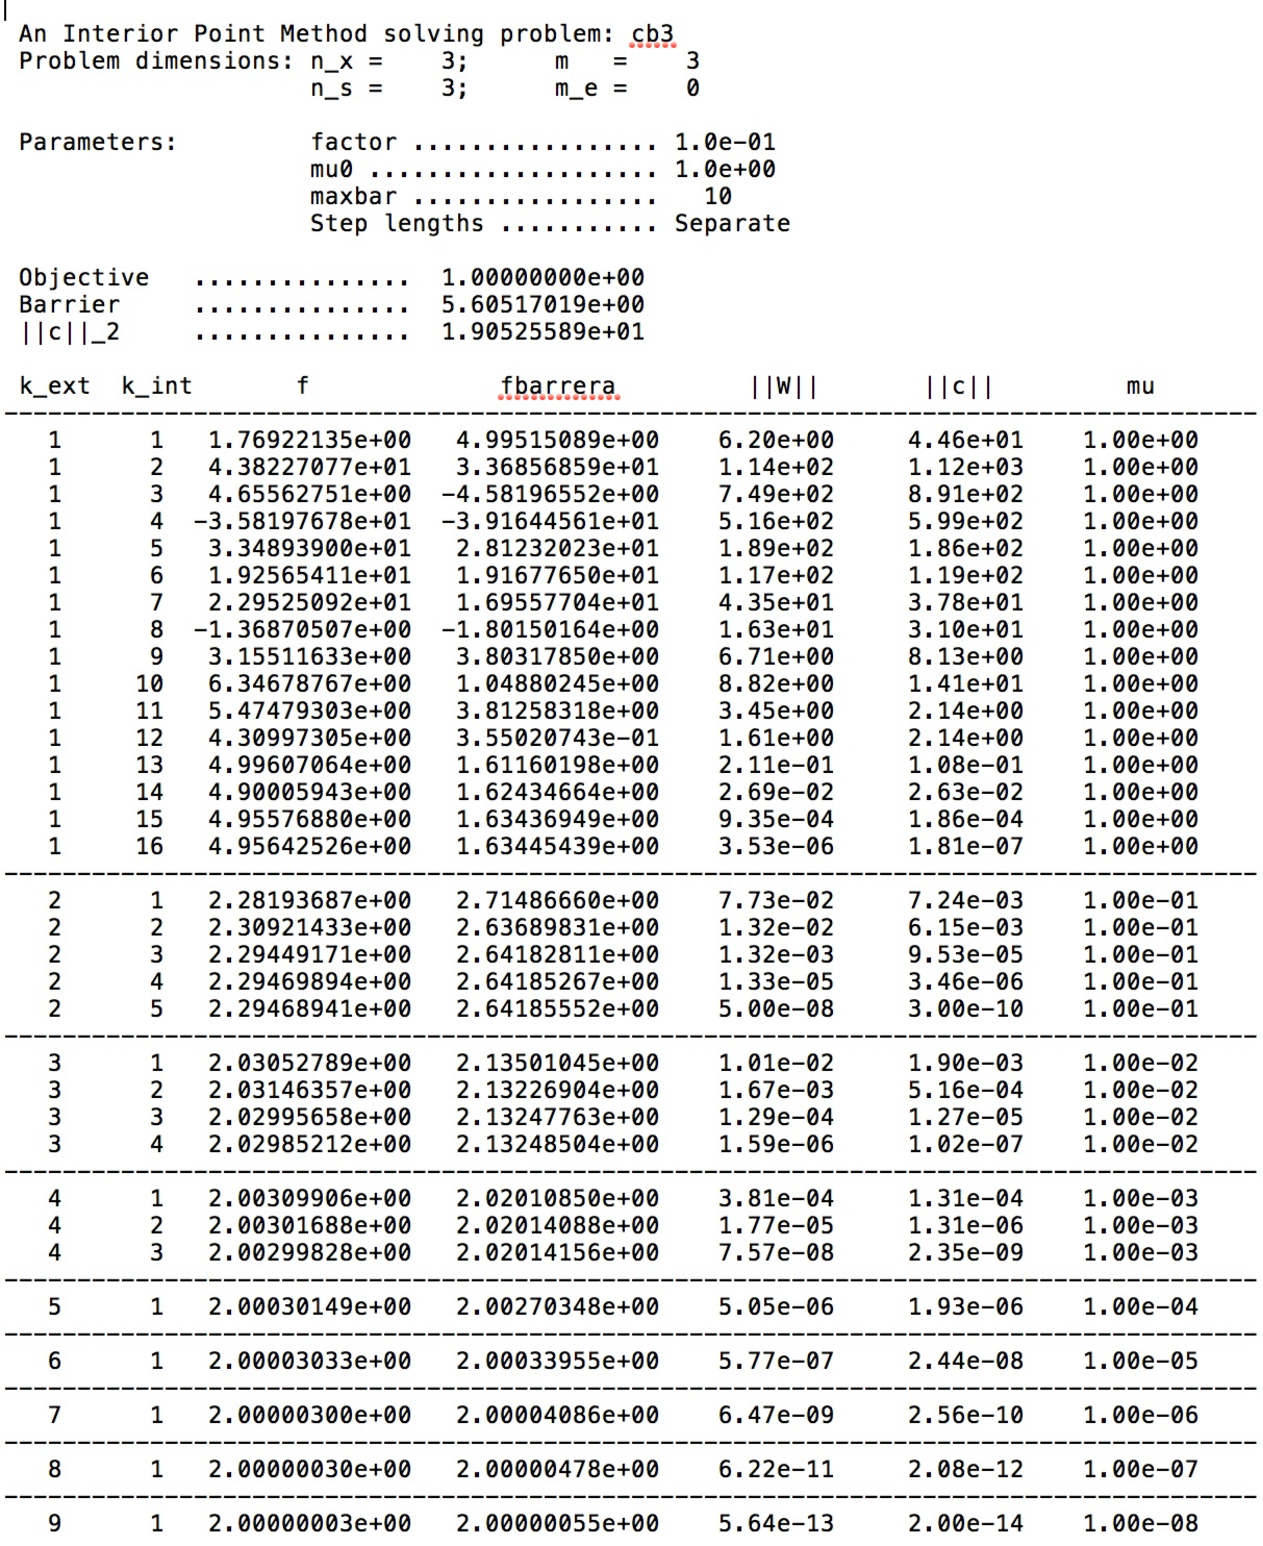
\includegraphics[trim=0 0 0 0,scale = 0.65]{cb3}
\end{figure}
\end{center}
\bei
\item Por \'ultimo, es importante hacer notar que la funci\'on de barrera va tendiendo a la funci\'on original $f$ conforme el valor de $\mu$ va disminuyendo. 
\eni
\pagebreak
\begin{center}
\begin{figure}[h]
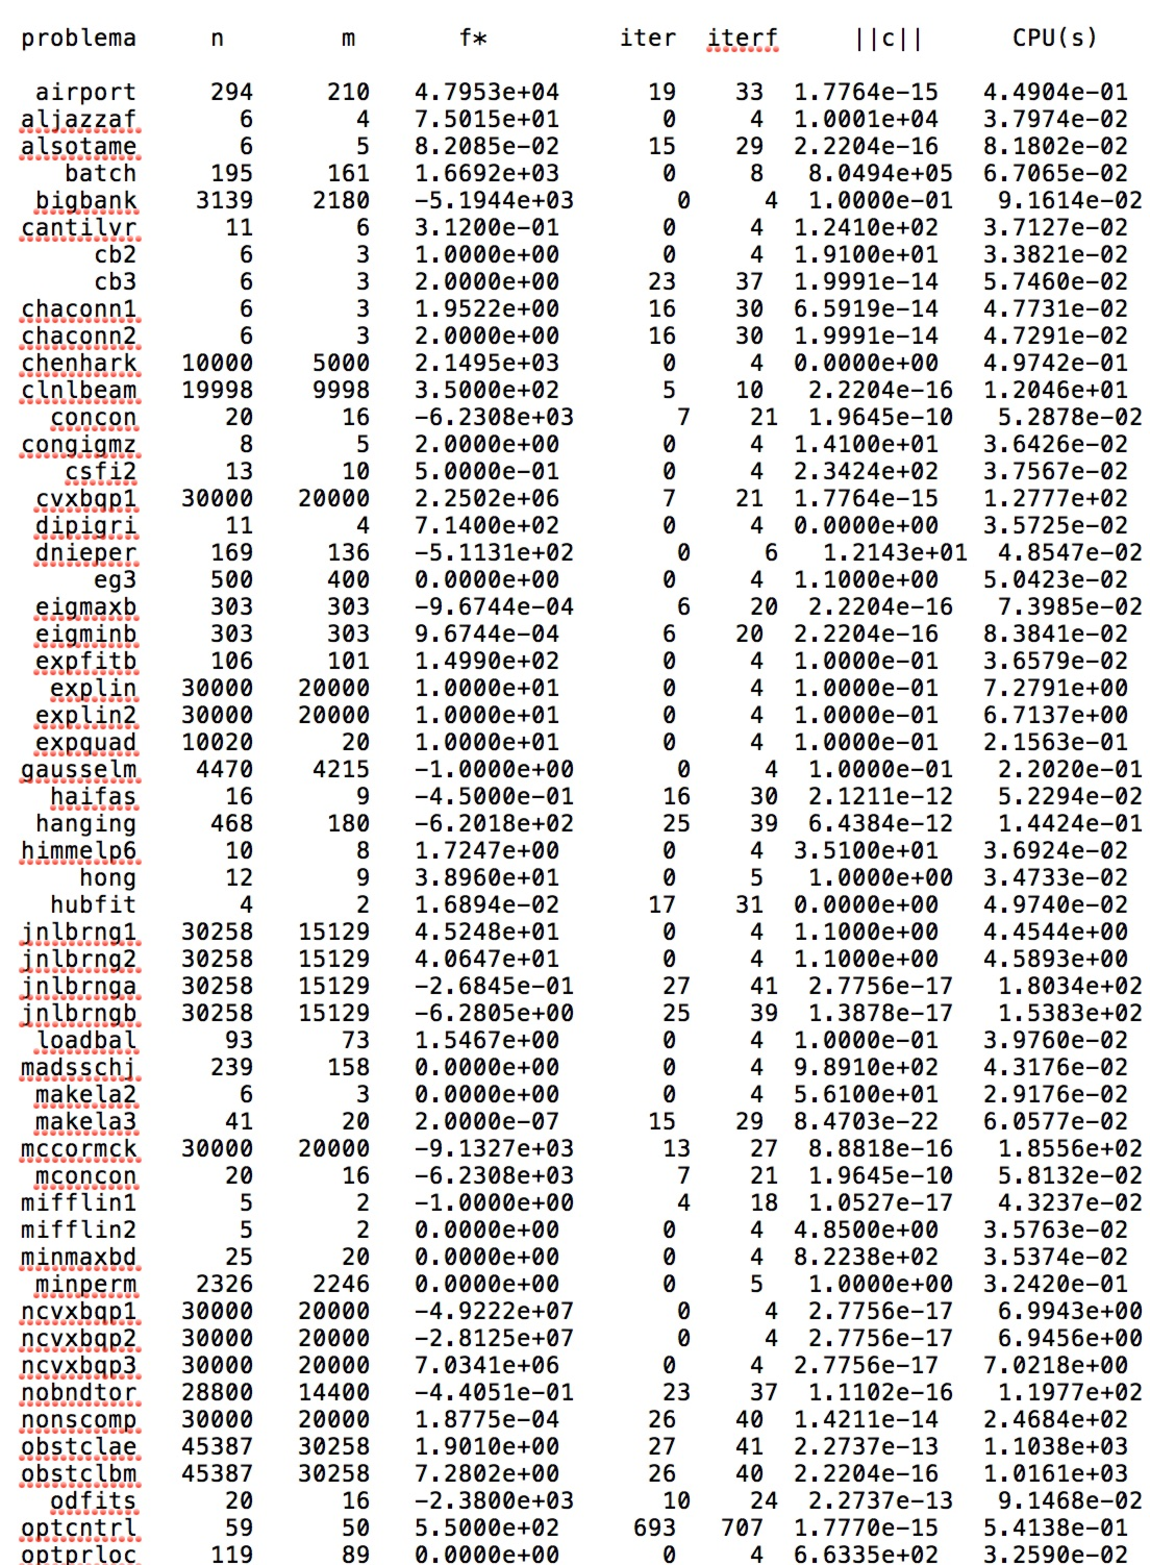
\includegraphics[trim=0 0 0 0,scale = 0.85]{problemas}
\end{figure}
\end{center}
\subsubsection*{Conclusiones}
\bei
\item Aunque por alg\'un tiempo los m\'etodos de puntos interiores perdieron terreno contra otro tipo de algoritmos como lo es el PCS, actualmente compiten muy bien contra cualquier algoritmo aunque su proceso sea diferente a los de los dem\'as (huir de la frontera en lugar de seguirla).
\item De una base de datos grande varios problemas no pudieron correr completamente (por inercia incorrecta la mayor\'ia), sin embargo este tipo de problemas pueden ser tratados como en PCS + RC para impulsar al algortimo a tener una convergencia global. 
\item A\'un en problemas de gran escala, los m\'etodos MPI pudieron dar resultados haciendo a veces menos de 23 iteraciones para problemas de tama�os en las decenas de miles. Eso es un gran poder de resoluci\'on para un algoritmo tan sencillo como lo es el de barrera logar\'itmica.
\item El siguiente paso a seguir podr\'ia ser incluir alg\'un tipo de separaci\'on en el programa que pudiera permitir usar MPI si el problema lo indica o PCS +GC con regiones de confianza si la curvatura no es correcta. 
\eni

\end{document}  